\chapter{EEG/MEG preprocessing --- Tutorial}
\label{ch:eeg_tutorial}
This tutorial will give a users guide to the pre-processing sections
of SPM M/EEG. We will use an example data set collected on a 128 active
electrode Biosemi EEG system. This data set is available from the SPM
website. The data was recorded continuously and had three event types
(event identifiers 1,2 and 4) These event types indicated the type of
visual stimulus presented.

\section{ERP analysis}

\subsection{Convert}
Convert reads the EEG data file and writes the data in a format that
is used for SPM analysis. The SPM format has two components a *.mat
and *.dat file. The *.mat file contains the data structure D and the
*.dat is the M/EEG data.\\

After clicking on Convert you will be asked to select the format of
your EEG or MEG data. For the example data set we select BDF. Next
select the data file. For the example data we select the
EEGexample.bdf. Next select the data template file from the EEG
template file. This file contains a template of electrode positions in
2D. For the example data set select the bdf\_setup.mat.\\

NB the questions then asked depend upon the data format selected. Here
we will only address the questions for the BDF format of the example
data set. 

For BDF files the HEOG, VEOG and any other additional recordings are
saved in the EXG channels. Here we attribute labels to these
recordings. For the example data set we recorded HEOG (EXG 3 4), VEOG
(EXG 4 5) and recorded from the earlobes (EXG 1 2) to allow
re-referencing offline. No other additional data were
recorded. Therefore we enter the following:

\begin{figure}
\begin{center}
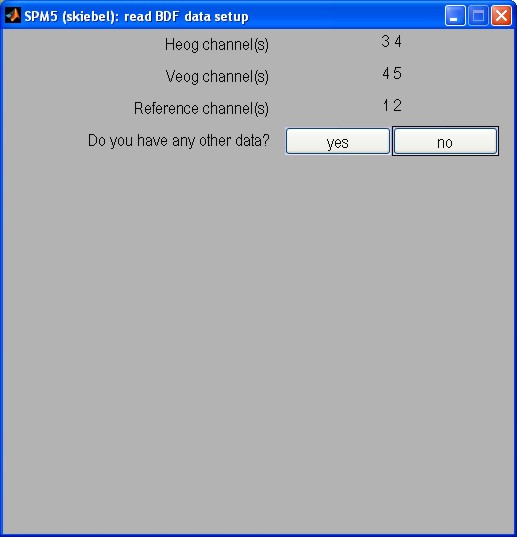
\includegraphics[width=100mm]{meeg/tutorial1}
\end{center}
\caption{\em Specifying the options for converting bdf-files} 
\end{figure}

The Convert function writes an EEGexample.mat and an EEGexample.dat
file in the current directory.

\subsection{Epoch}
To epoch the data click on epoching. Select the EEG mat file to
epoch. Choose the peri-stimulus time window. Choose the events to
epoch. Possible events will be listed in the Matlab command window. If
you do not have any events in you converted data file you can input
them in by reading in a new event list.

For the example data set exampleEEG.mat was selected and the following
parameters were used:

\begin{figure}
\begin{center}
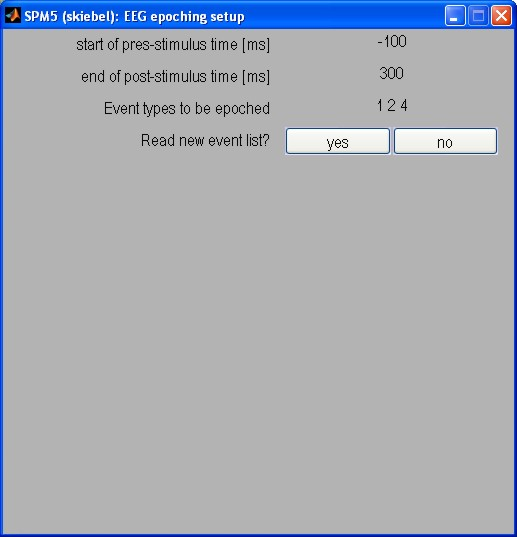
\includegraphics[width=100mm]{meeg/tutorial2}
\end{center}
\caption{\em Specifying the options for epoching the example data} 
\end{figure}

Having epoched the data one could filter and downsample the epoched data as above.
Epoching writes a *.mat and *.dat file prefixed by a 'e\_'. 

\subsection{Filter}
Filter filters the data using a Butterworth filter. This can be
applied either before or after epoching (see 1.3). Here it is applied
after. 

After clicking Filter select the *.mat file produced by Convert. For
the example data set select e\_EEGexample.mat. 

Next select the filter type, either lowpass or bandpass. If lowpass is
selected enter the cut-off frequency. If bandpass is selected enter
the two frequencies that specify the band of interest. \\ 

The Filter function writes a *.mat and *.dat file prefixed by a 'f'. \\

For the example data set e\_exampleEEG.mat was selected and a bandpass
filter was used from 0.1-45 Hz.


\subsection{Downsample}
To downsample the data select downsample from the 'Other' pull-down
menu. Select the data file to downsample. Enter the new sampling
rate. For the example dataset we downsampled to 100 Hz. Downsample
writes a *.mat and *.dat file prefixed by a 'd'.

For the example data set fe\_exampleEEG.mat was selected.

\subsection{Artefacts}
Two different methods of artefact removal are implemented in SPM5. One
is a simple thresholding method. The other uses a robust averaging
methodology to weight each time point by a function of the residuals. 

To remove artefacts click on Artefacts. Select the epoched data file
to analyse. If you know of bad trials or electrodes that you noted
during acquisition or found using another methodology you can read
them in using the 'read own artefact list'. If you want to use robust
averaging click yes to the following question if not click no. To
threshold channels click yes and then enter the threshold you wish to
use. The thresholding has two passes. One to find bad electrodes and
the second to find bad trials. If robust averaging was selected the
second pass will apply the robust averaging approach but a first pass
could use a thresholding method to find the bad electrodes prior to
robust averaging.\\

Artefacts writes a *.mat and *.dat file prefixed by an 'a'.\\ 

\begin{figure}
\begin{center}
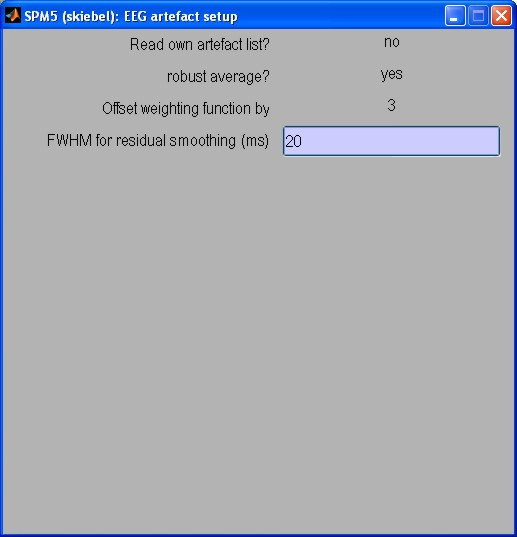
\includegraphics[width=100mm]{meeg/tutorial3}
\end{center}
\caption{\em Specifying the options for artefact detection in the
  example data}
\end{figure}

For the example data set dfe\_exampleEEG.mat was selected. No artefact
list was used and robust averaging was selected with a threshold of
100  v. For the robust averaging the default parameters were used.

\subsection{Averaging}
To produce a mean ERP click on averaging and select the EEG mat file
that you wish to average. This will automatically average either
ignoring the bad channels and trials or it will apply the weighting
matrix calculated from robust averaging. For the example data set
adfe\_exampleEEG.mat was selected.\\

Averaging writes a *.mat and *.dat file prefixed by an 'm'. 

\section{Other useful functions}
\subsection{Time-Frequency}
In SPM5 it is possible to apply a time-frequency analysis to the
data. This can either be applied to the averaged ERP to produce
time-frequency plot of evoked oscillations. Or it can be applied to
each trial and then averaged across trials to produce time-frequency
plot of evoked oscillations and induced oscillations. To produce
time-frequency plots select time-frequency from the other pull-down
menu. Select the EEG mat file to analyse. Enter a vector containing
the frequencies that you wish to analyse. You are then given the
option to baseline correct the time-frequency data. Next enter the
Morlet wavelet factor that you wish to use. The default value is
7. Next you can select the channels you wish to analyse. The default
is all channels.\\

Time-Frequency writes two *.mat and *.dat files. The first, the power,
is prefixed by 't1'. The second, the phase, is  prefixed by 't2'.

\subsection{Average TF}
To average time-frequency data sets across trials select average TF
from the other pull down menu. Select the T1*.mat EEG mat file to
average. As with the Averaging function Average TF writes a *.mat and
*.dat file prefixed by an 'm'.